\section{Performance Evaluation}
\subsection{Efficacy of the ODE model}
\label{subsec:pe_valid}
\begin{figure}
  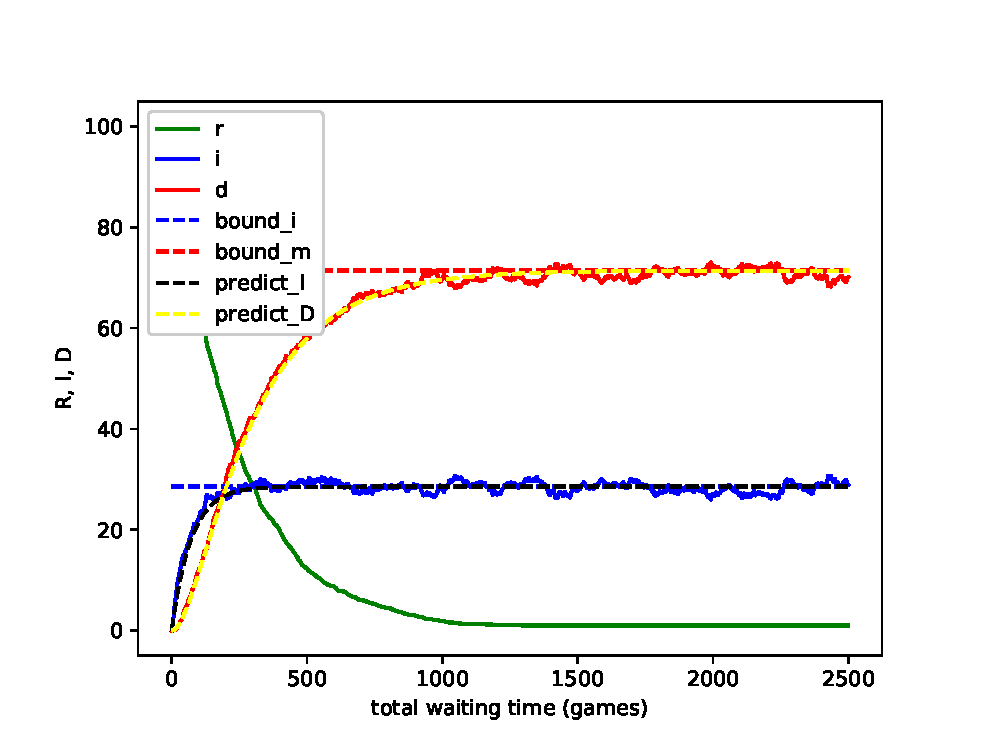
\includegraphics[width=.45\textwidth]{fig/twohop_without_detection.eps}
  \caption{$I(t)$, $D(t)$ and $R(t)$ with time computed from prediction and simulations when $\lambda = 0.004$, $\rho = 0.01$, $N=100$ and $T=2,500$.}
  \label{fig:twohop_predict_wod}
\end{figure}
Fig.~\ref{fig:twohop_predict_wod} shows that the change of the states
in the experiments conforms to the solved solutions (\ref{eq:IDR_wo_solu}).
Here $D(t)$, $I(t)$ and $R(t)$ are the mean values 
at the specific time $t$ of $20$ simulations.
[*** add $R(t)$ ***]
[*** add J P p ***]

\subsection{Efficacy of the approximate method}
Fig. XX shows the approximate ratio of (\ref{eq:IDR_full}).

\subsection{Optimal solution}
\begin{figure}
  \centering
  {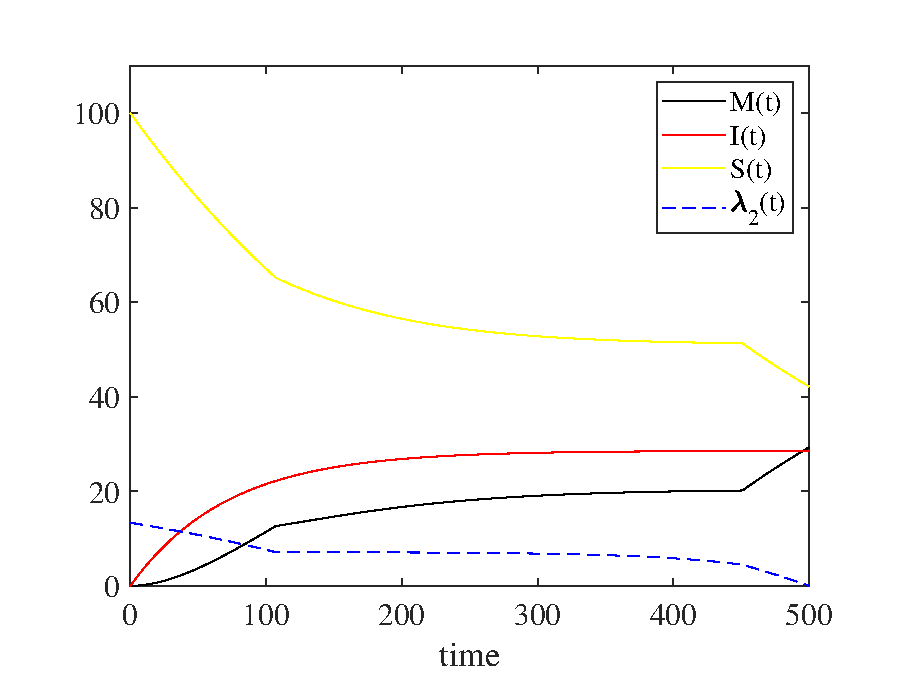
\includegraphics[width=0.47\textwidth]{fig/state.eps}}
     \caption{State variable of analysis with time.}
     \label{fig:pe_opt_state_time}
\end{figure}
\begin{figure}
  \centering
  {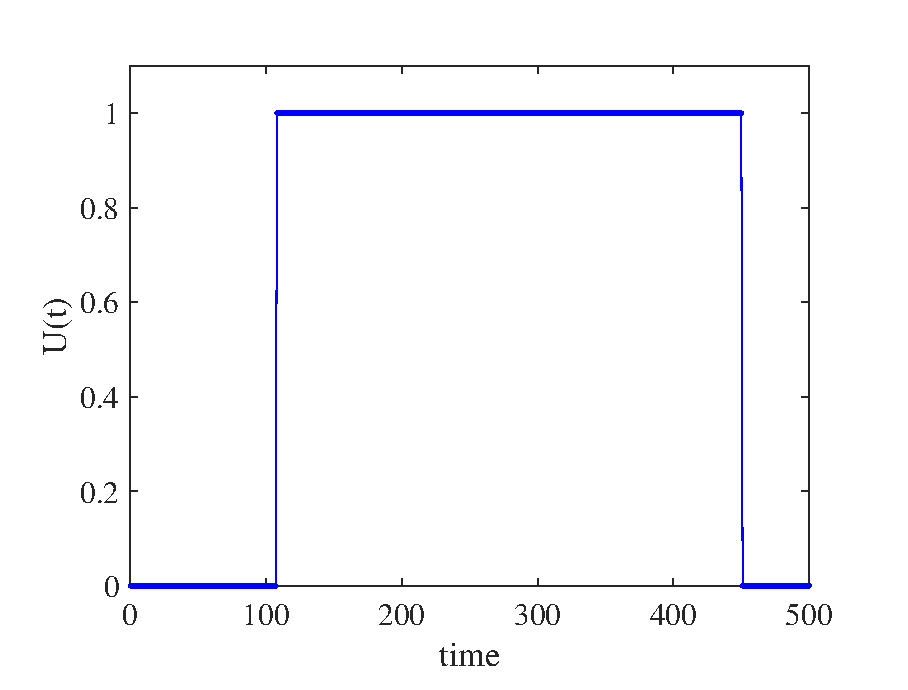
\includegraphics[width=0.47\textwidth]{fig/Ut.eps}}
     \caption{Control variable of analysis with time.}
     \label{fig:pe_opt_control_Ut}
\end{figure}
\begin{figure}
  \centering
  {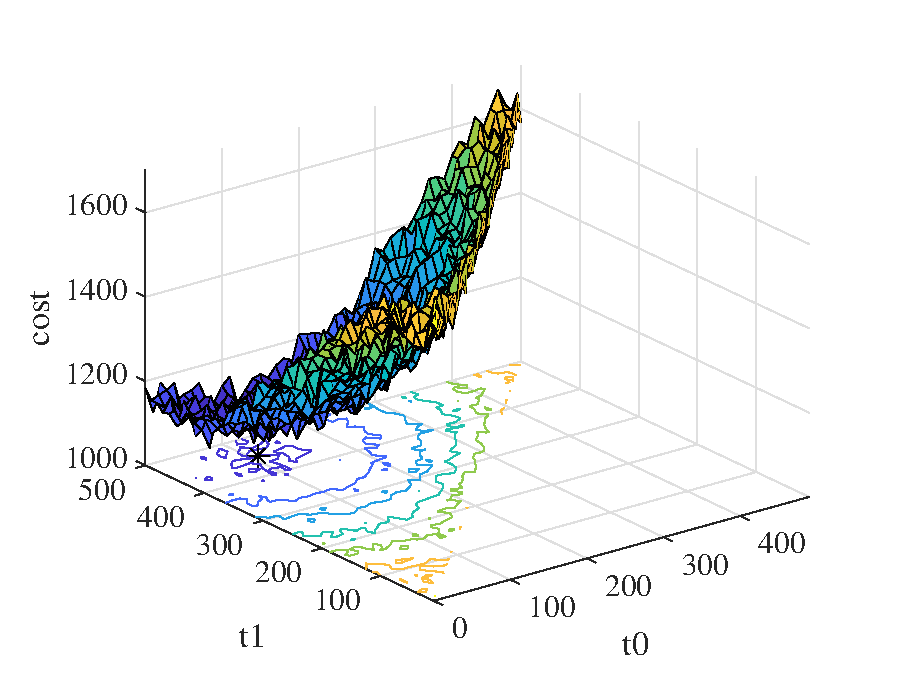
\includegraphics[width=0.47\textwidth]{fig/cost_all_t0t1.eps}}
     \caption{Different choices of $t0$ and $t1$.}
     \label{fig:pe_diff_choices}
\end{figure}
